\documentclass[tikz,border=2pt]{standalone}
\usepackage{amsmath,amssymb}
\usepackage{tikz}
\usetikzlibrary{arrows.meta}

\begin{document}
% Exogenous variables x are set from outside; the equation system F(x, y) = 0 then determines
% the endogenous variables y = g(x) (locally, by the implicit function theorem).
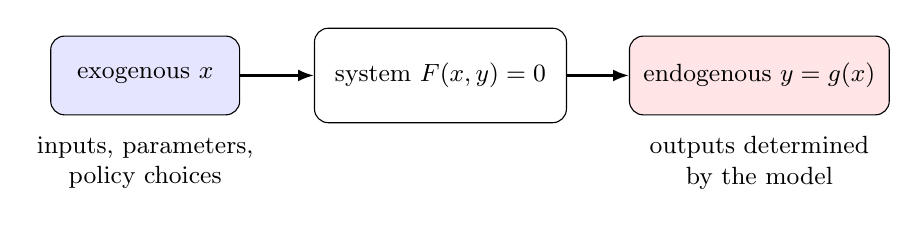
\begin{tikzpicture}[every node/.style={font=\small}, >={Latex[length=2mm]}]
	\node[draw, rounded corners=5pt, fill=blue!10, minimum width=2.4cm, minimum height=1cm] (x) at (0,0) {exogenous $x$};
	\node[draw, rounded corners=5pt, minimum width=3.2cm, minimum height=1.2cm] (F) at (3.75,0) {system $F(x,y)=0$};
	\node[draw, rounded corners=5pt, fill=red!10, minimum width=3.3cm, minimum height=1cm] (y) at (7.8,0) {endogenous $y=g(x)$};
	\draw[->, thick] (x) -- (F);
	\draw[->, thick] (F) -- (y);
	\node[anchor=north, align=center] at (0,-0.65) {inputs, parameters,\\ policy choices};
	\node[anchor=north, align=center] at (7.8,-0.65) {outputs determined\\ by the model};
\end{tikzpicture}
\end{document}
